\question{}

\begin{ابجد}
\item اگر برای تعیین ارزش گره‌های \lr{CHANCE}، مقدار امید ریاضی ارزش آنها را حساب کنیم، ارزش گره‌ها به این صورت خواهد بود:
\begin{figure}[H]
    \centering
    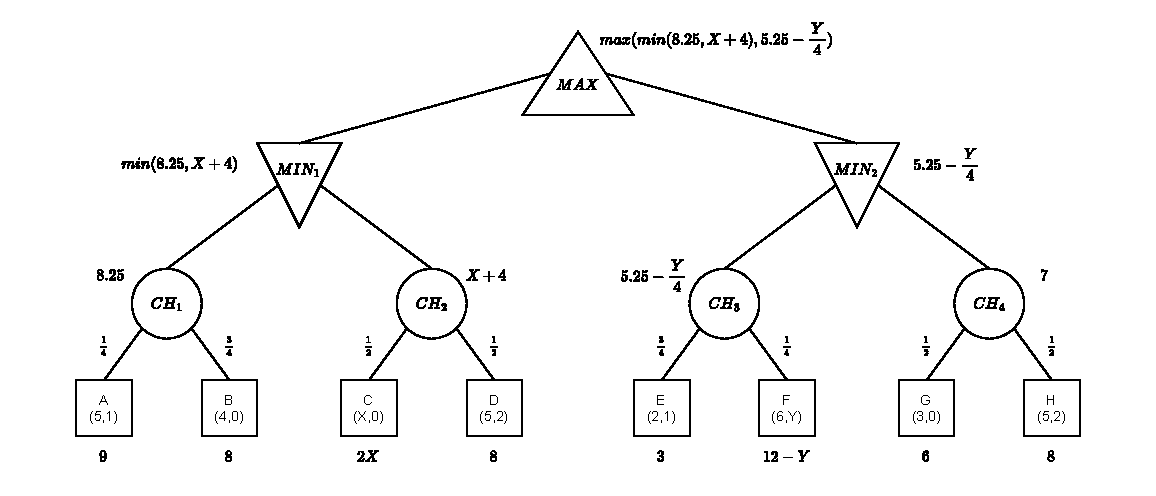
\includegraphics[width=0.9\textwidth]{assets/q2-A.pdf}
\end{figure}
توجه داریم که $v(MIN_2) = \min(5.25 - \frac{Y}{4}, 7) = 5.25 - \frac{Y}{4}$

\item در این حالت درخت به این شکل خواهد بود:
\begin{figure}[H]
    \centering
    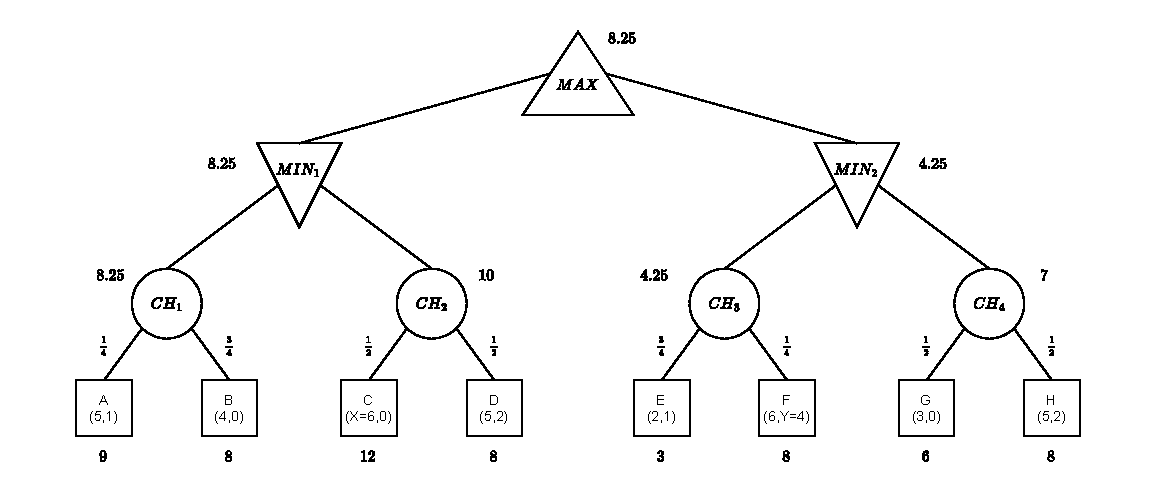
\includegraphics[width=0.9\textwidth]{assets/q2-B.pdf}
\end{figure}
همان طور که مشاهده می‌شود، $v(MIN_1)=8.25$ و $v(MIN_2)=4.25$. بنابراین بازیکن $MAX$ که به دنبال بیشینه کردن امتیاز است، در ریشه، شاخه سمت چپ را انتخاب می‌کند.

\item همان طور که در بخش اول محاسبه کردیم:
\begin{align*}
     & v(MIN_1) = \min(8.25, X+4)    \\
     & v(MIN_2) = 5.25 - \frac{Y}{4}
\end{align*}
بنابراین اگر بخواهیم بازیکن $MAX$ شاخه سمت راست را انتخاب کند، داریم:
\begin{align*}
    v(MIN_2) > v(MIN_1)  \Rightarrow                             & 5.25 - \frac{Y}{4} > \min(8.25, X+4)                           \\
    \xRightarrow{Y \geq 0 \Rightarrow 5.25 - \frac{Y}{4} < 8.25} & X+4 < 8.25 \quad \land \quad X+4 < 5.25 - \frac{Y}{4}          \\
    \Rightarrow                                                  & X < 4.25 \quad \land \quad X+ \frac{Y}{4} < 1.25               \\
    \Rightarrow                                                  & (X,Y) \in \{ (0, 0), (0, 1), (0, 2), (0, 3), (0, 4), (1, 0) \}
\end{align*}
و اگر بخواهیم ارزش دو شاخه برابر شود:
\begin{align*}
    v(MIN_2) = v(MIN_1) & \Rightarrow 5.25 - \frac{Y}{4} = \min(8.25, X+4)                  \\
                        & \Rightarrow X+4 < 8.25 \quad \land \quad X+4 = 5.25 - \frac{Y}{4} \\
                        & \Rightarrow X < 4.25 \quad \land \quad X+ \frac{Y}{4} = 1.25      \\
                        & \Rightarrow (X,Y) \in \{ (0, 5), (1, 1) \}
\end{align*}

\item طبق فرض سوال هرس تنها در گره‌های $MIN/MAX$ انجام می‌شود، بنابراین تا قبل از اینکه گره $MAX$ مقداردهی اولیه نشده باشد، نمی‌توانیم گرهی را هرس کنیم. پس باید صبر کنیم تا گره‌های $A$، $B$، $C$ و $D$ دیده شوند. در این حالت:
\begin{equation*}
    v(CH_1) = 8.25, \quad v(CH_2) = 10, \quad v(MIN_1) = 8.25, \quad v(MAX) = 8.25
\end{equation*}
حال می‌توانیم به زیرگره سمت راست برویم. مشابه قسمت قبل برای اینکه بتوانیم گرهی را هرس کنیم، ابتدا باید $MIN_2$ مقداردهی شده باشد، پس باید $CH_3$ مقدار داشته باشد و در نتیجه $E$ و $F$ دیده شده‌اند. در این حالت می‌دانیم که $v(MIN_2) \leq v(CH_3) = 4.25$. از آنجا که $v(MAX)=8.25$ و $v(MAX) > v(MIN_2)$، نیازی به دیدن گره‌های $G$ و $H$ و محاسبه ارزش $CH_4$ نداریم، چون به هر حال بازیکن $MAX$ مسیر سمت راست را انتخاب نمی‌کند. \\
بنابراین زیردرخت $CH_4$ (شامل برگ‌های $G$ و $H$) هرس می‌شود.

\end{ابجد}